\documentclass{article}
\usepackage{amsmath}
\usepackage{float}
\usepackage{graphicx}
\usepackage{geometry}
\usepackage{tabularx}
\begin{document}
\title{Problem Set 9}
\author{Xin Gao}
\date{}
\maketitle

\section{Final Project Abstract and Figures}
Recent scientific efforts have observed ejection of ice plumes from
geysers in the south polar region of Enceladus, a moon of Saturn. The
likelihood of the existence of cryovolcanoes inside Enceladus along with
planetary modeling along with other lines evidence suggests the presence
of a liquid water ocean beneath the Enceladus. How likely is it for such
an ocean to actually exist and can Enceladus live up to its name as the
prime candidate for possibly hosting extraterrestrial life?

\begin{figure}[H]
\centering
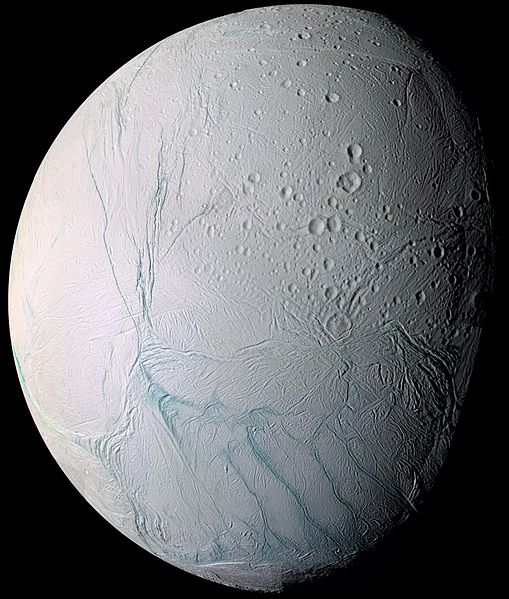
\includegraphics[width=.6\textwidth,height=4in]{enceladus_stripes.png}
\caption{The infamous ridges of Enceladus shown here were first
  discovered by the Cassini-Huygens probe in 2005. The false-color lines
  denote the locations of the geysers from which ice was shown being
  spewn out and where ice and simple organic carbon compounds have been
  detected. Source: Wikipedia}
\end{figure}
\begin{figure}[H]
\centering
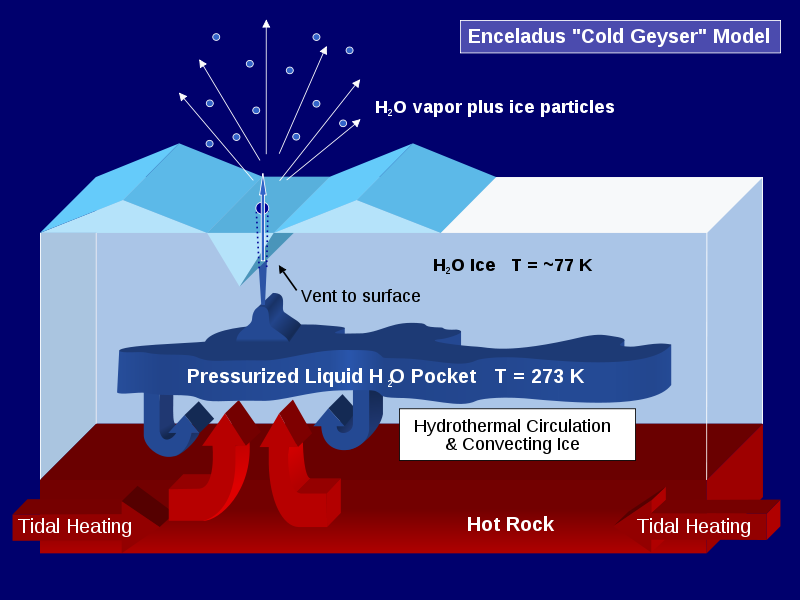
\includegraphics[width=.8\textwidth]{enceladus_geyser.png}
\caption{This diagram aims to explain the mechanism behind possible
  cryovolcanism and subsurface ocean. Tidal heating in the mantle, which
  can give rise to a geologically active subsurface world, likely exists
  due to Enceladus' position relative to Saturn and other moons of
  Saturn. The resulting circulation would produce the conditions for a
  liquid ocean water between the icy crust and the molten
  mantle. Source: Wikipedia} 
\end{figure}
\section{Magnetic Field Decay}
See attached paper.
\section{Pluto-Charon}
See attached paper.
\section{Science News Reporting}
a. $www.sciencenews.org/article/speed-early-universe's-expansion-determined$
b. 2-3 sentences $/$ paragraph
c. Astronomers used the radial velocities of early dust clouds,
illuminated by background quasars, to determine the rate of expansion,
with relative accuracy, of the universe when gravity was deccelerating
the expansion rate.  
\end{document}
